\subsection{Flow based solutions}

We can solve instances of $\Problem$ where the properties $cv$, $bw$, $r$ and 
$ma$
are present, by reducing it to a series of flow problems on an extended 
host graph. We utilize the following observations:

\newcommand{\Source}{\ensuremath{s}}
\newcommand{\Sink}{\ensuremath{t}}

\begin{enumerate}
\item $cv$ + $bw$ + $r$ + $ma$ degenerates to  $bw$ + $r$ + $ma$. 
The placement of the VMs is given. The bandwdith function $\Capacity$ assigns 
each edge in the host graph $\SubstrateEdge_i$ a capacity 
$\Capacity(\SubstrateEdge_i)$. Since the 
host graph is a tree, there exists only one path between two nodes, and hence 
it is known how much bandwidth has to be allocated on which links, in oder to 
satisfy the communication between the VMs. We can therefore construct a 
problem with $bw$ + $r$ + $ma$ which has the same solutions, by defining 
$\Capacity'(\SubstrateEdge_i)$ as 
$\Capacity(\SubstrateEdge_i) - \textsc{CV}(\SubstrateEdge_i)$, where 
$\textsc{CV}(\SubstrateEdge_i)$ denotes the amount which 
had to be allocated on the link $\SubstrateEdge_i$ for the communication 
between the $\VM s$. If any of the resulting edge capacities is negative, the 
instance of $\Problem$ is infeasible.
\item The required bandwidth $\CostTrans$ between each chosen chunk and the 
assigned VM of a given $\VC$ is 
the same and the pathes to the VMs have to be embedded as unsplittable 
pathes.

TODO: rethink if normalization allows solving the problem by integer min-cost-max flow

Hence, all edge capacities in can be normalized to $\CostTrans = 1$.
\item For a (by model) fixed node mapping $\NodeMapping$ and a given chunks to 
vm assignment $\VmChunkAssignment$, the computation of a cost 
optimal link mapping can be transformed to an integral minimal cost multi-commodity 
flow problem, where each VM $\VirtualNode_i$ has a flow demand of $1$ to each 
of its assigned chunks $\VmChunkAssignment(\VirtualNode_i)$. This problem can 
again be transformed into a integral minimum cost single commodity flow problem 
in the following way: 
We introduce a 
super source $\Source$ and edges $\SubstrateEdge_i^+ = (\Source, 
\NodeMapping(\VM_i))$ for 
$i \in \{1,\dots,\Vms\}$ with $\Capacity(\SubstrateEdge_i^+) = \MaFactor$, 
which connects $\Source$ 
to the nodes in the host graph, on which the VMs are located. 
In addition we create a super sink $\Sink$ and edges $\SubstrateEdge_j^- = 
(\VmChunkAssignment(\ChunkLocation(\Chunk_j)), \Sink)$ with capacities 
$\Capacity(\SubstrateEdge_j^-) = 1$, which connect the leaves on which the 
chunks are located to the sink. In this graph we ask for a flow $f$ 
of value $\ChunkTypes$ from $\Source$ to $\Sink$. \carlo{TODO: The 
equivalency...}
\item The replica selection problem can be integrated into the above described 
minimum cost integral single commodity flow problem. Since $\VmChunkAssignment$ 
is not given, but subject to optimization, the edges connecting $\Sink$ to the 
chosen chunks are no longer implementable. Instead, we create a meta node 
$\SubstrateNode_{\Chunk_j}$ for each chunk type 
$\Chunk_j$ and connect it with \carlo{TODO Check directed?!?} edges 
$\SubstrateEdge_{\Chunk_j}^k = (\SubstrateNode_{\Chunk_j}, 
\VmChunkAssignment(\Chunk_{j_k}))$ for all $k \in 
\{1,\dots,\RedundancyFactor\}$. Subsequently we connect the super sink 
$\Sink$ to these meta nodes, via 
edges $\SubstrateEdge_j^- = (\SubstrateNode)$ with 
$\Capacity(\SubstrateEdge_j^-) = 1$. If an integral minimum cost flow $\hat f 
: \SubstrateEdges \rightarrow \mathbb{N}$ of value $\ChunkTypes$ exists, it 
enters the graph at leaves the graph at $\Sink$. Since the only 
edges which connect to $\Sink$ are introduced by our construction $\sum_{j\in 
\{1,\dots,\ChunkTypes\}} \hat f(\SubstrateEdge_j^-) = \ChunkTypes$ holds. From 
$\Capacity(\SubstrateEdge_j^-) = 1$, follows $\hat f(\SubstrateEdge_j^-) = 1 ~ 
\forall j \in \{1,\dots, \ChunkTypes\}$. Hence, for each chunk type $\Chunk_j$, 
$\sum_{k \in \{0,\dots,\RedundancyFactor\}}\hat f(\SubstrateEdge_{c_j}^k) = 1$ 
holds, which - due to the integral solution to the minimal cost flow problem -  
can be interpreted as the replica selection. $\hat f$ enters the graph at 
$\Source$ resulting in $\sum_{i \in \{1,\dots,\Vms\}}\hat f(\SubstrateEdge_i^+) 
= \ChunkTypes = \Vms \cdot \MaFactor$. Due to the capacity limitations this is 
equivalent to $\hat f(\SubstrateEdge_i^+) = \MaFactor ~ \forall i \in 
\{1,\dots, \Vms\}$, which represents $\MaFactor$ outgoing flows for each node 
in the host graph, to which a VM is assigned.
\item To compute $\VmChunkAssignment$ from $\hat f$, we process $\hat f$ in the 
following way: We chose an aribtrary path $\Path = 
\{\SubstrateEdge_{1}, \dots, \SubstrateEdge_{n}\}$, with $\SubstrateEdge_{1} = 
(\Source, \NodeMapping(\VirtualNode_i))$, $\SubstrateEdge_{n} = 
(\SubstrateNode_j, \Sink)$, $\SubstrateEdge_k= (\SubstrateNode_x, 
\SubstrateNode_y) \rightarrow \SubstrateEdge_{k+1} = (\SubstrateNode_y, 
\SubstrateNode_z)$, and $\hat f(\SubstrateEdge)\geq 1 ~ \forall \SubstrateEdge 
\in \Path$. This is a connected path from the source, to the sink, which has 
flow associated on every edge. We set $\VmChunkAssignment(\Chunk_j) = 
\VirtualNode_i$ and reduce $\hat f$ on every edge $\SubstrateEdge \in \Path$ by 
one. This is repeated, until $|\hat f| = 0$. Due to the tree properties of 
$\Tree$, that there is only one path between two nodes, all VM chunk 
assignments generated in this value will have the same overall costs.

\begin{comment}
\item For a given chunk \textit{type} to VM assignment, the replica selection 
problem 
can be integrated into this problem, by introducing nodes 
$\SubstrateNode_\ChunkType$ for each 
chunk type $\ChunkType$ and connect these nodes via edges 
$\SubstrateEdge_\ChunkType = (\SubstrateNode_\ChunkTypes, \SubstrateNode_i)$ 
for all $i$ such that \carlo{Check macieks part for assigned = true}. The 
capacity of all of these edges is set to 
$\Capacity(\SubstrateEdge_\ChunkTypes) = 1$. In this problem 
%
This problem can be converted into 
a integral minimum cost single commodity flow problem, 
%
In addition we create a super sink 
$\Sink$ and edges 
$\SubstrateEdge_\ChunkType^-$ with $\Capacity(\SubstrateEdge_\ChunkType^-) = 1$
%
\item The chunk to vm assignment decision, can be 
integrated into the above described flow problem, by transforming it into a 
integral minimum cost single commodity flow problem.
We introduce a super source $\Source$ and edges $\SubstrateEdge_i^+ = (\Source, 
\NodeMapping(\VM_i))$ for $i \in \{1,\dots,\Vms}$ with 
$\Capacity(\SubstrateEdge_i^+) = \MaFactor$, which 
connects $\Source$ to the nodes in the host graph, to which the VMs are mapped. 
In addition we create a super sink $\Sink$ and edges 
$\SubstrateEdge_\ChunkType^-$ with $\Capacity(\SubstrateEdge_\ChunkType^-) = 1$
%
We extend the flow graph with a nodes $\SubstrateNode_\ChunkType$ for each 
chunk type $\ChunkType$ and connect these nodes via edges 
$\SubstrateEdge_\ChunkType = (\SubstrateNode_\ChunkTypes, \SubstrateNode_i)$ 
for all $i$ such that \carlo{Check macieks part for assigned = true}. The 
capacity of all of these edges is set to 
$\Capacity(\SubstrateEdge_\ChunkTypes) = 1$.
In addition we create a super sink $\Sink$ and edges 
$\SubstrateEdge_\ChunkType^-$ with $\Capacity(\SubstrateEdge_\ChunkType^-) = 
1$, to connect the meta nodes for each chunk type to the super sink.
%Instead of connecting 
%$\Source$ to the nodes, to which the VMs are mapped, we connect $\Source$ to 
%\textit{all leaves} in the host graph via edges $e_\Leaf^+ = (\Source, 
%\SubstrateNode)$. $\Capacity(e_\SubstrateNode^+)$ is set to one, since by 
%the definition of our model, only one VM may be mapped to one server. If a 
%feasible flow $f : \SubstrateEdges \rightarrow \mathbb{N}$ of value $\Vms$ 
%exists, then $\Sum_{\Leaf \in \Leaves}$
\end{comment}
\end{enumerate}

\begin{figure}
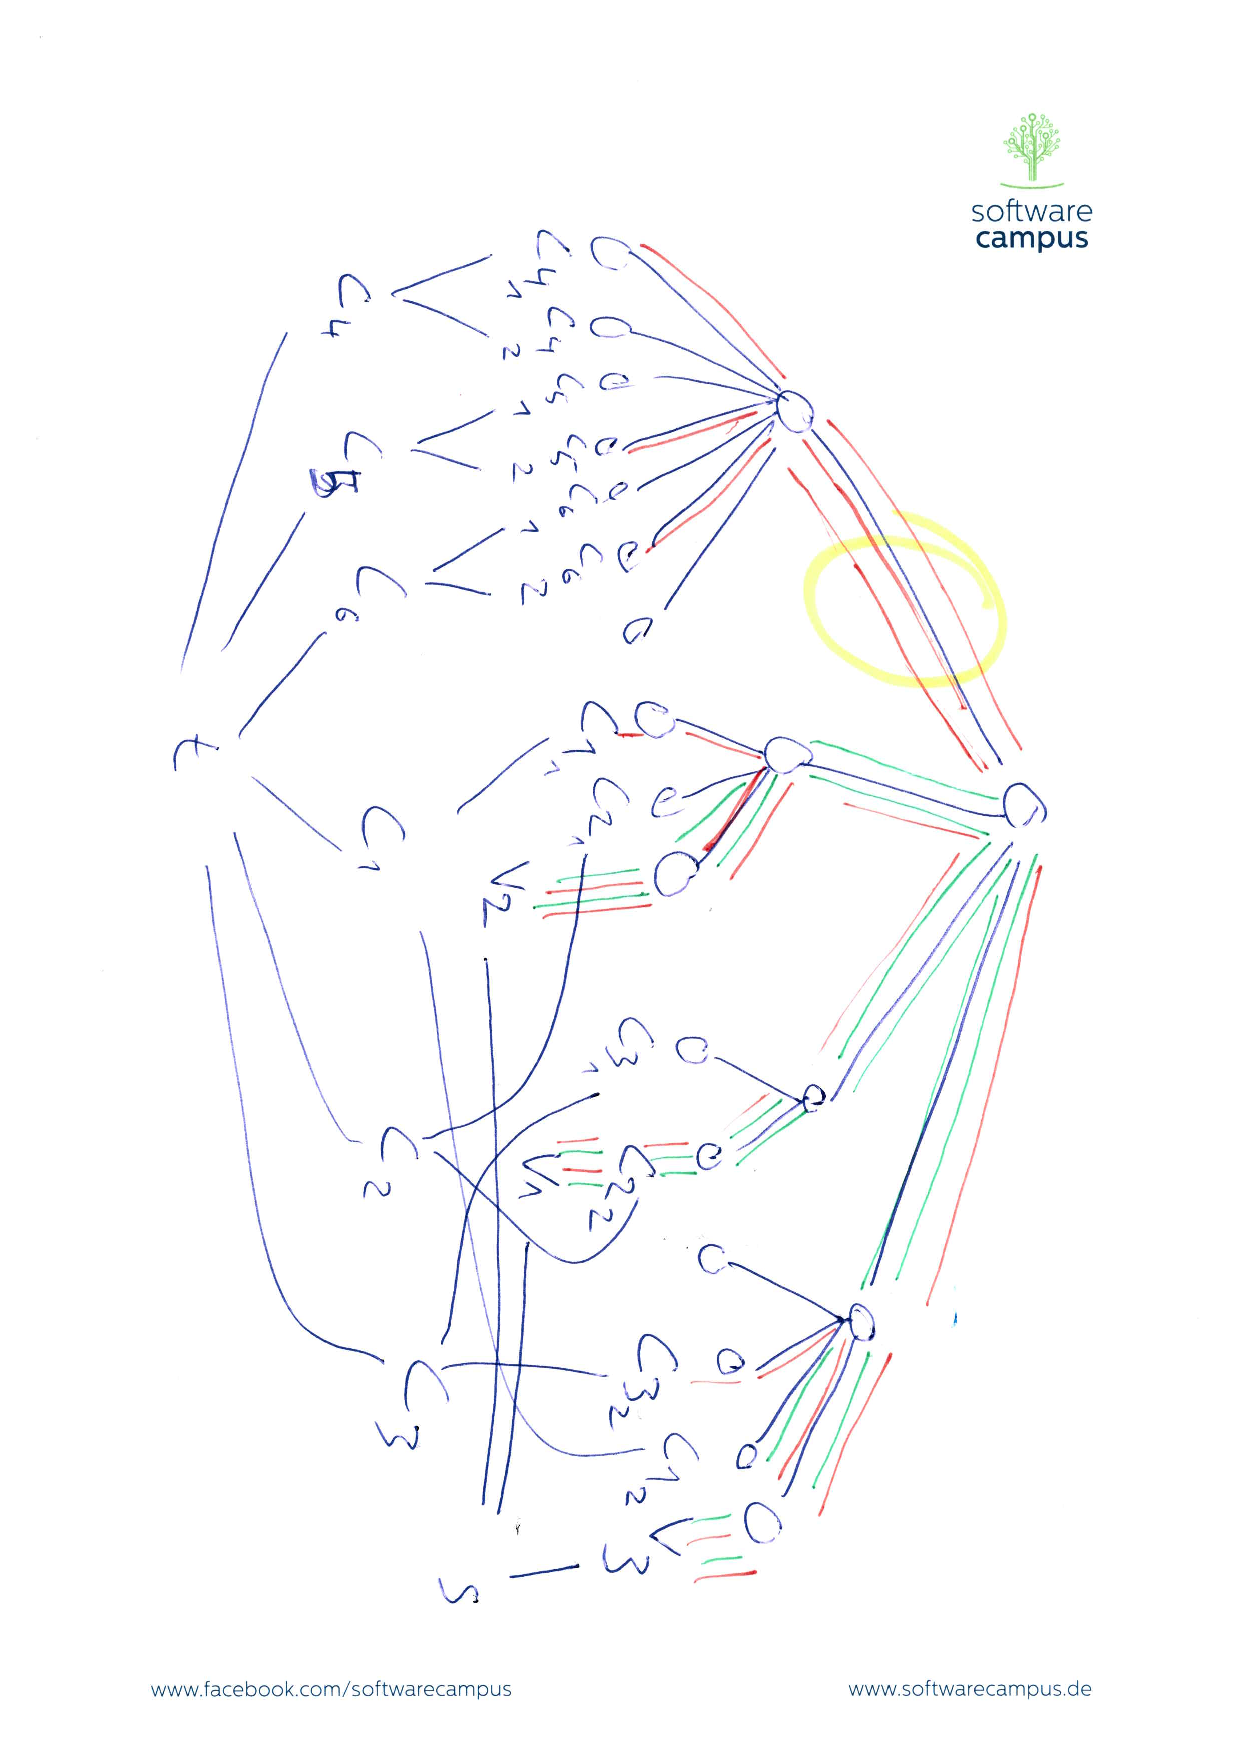
\includegraphics[angle=90,origin=c, height=7cm]{figs/model_fig_skteches/flow}
\end{figure}


Many algorithm can compute a solution for the integral minimum cost maximum 
flow problem. One example is the \textit{successive shortest path algorithm}, 
which can compute a solution in $\mathcal{O}(n \cdot U((n+m)\log n)
)$ time \cite{successive_shortest_path_complexity}, where $n$ is the number of 
nodes in the flow graph ($|\SubstrateNodes| + \ChunkTypes$), $m$ is the number 
of edges in the substrate graph ($|\SubstrateEdges| + \Vms + \RedundancyFactor 
\cdot \ChunkTypes$) and $U$ is the highest capacity in the substrate 
($\max(\Capacity(\SubstrateEdge))~\SubstrateEdge\in\SubstrateEdges$).




\begin{comment}
\paragraph{FLOW Construction}

This section presents a flow based solution for the variant of the model which 
has bandwidth limitations, communicatin between the $\VM s$ and redundant 
$\Chunk s$.

We start by showing that $cv$ + $bw$ + $r$ is the same problem as $bw$ + $r$. 
The placement of the $\VM s$ is given. The bandwdith function $b$ assigns 
each link in the physical substrate $l_i$ a capacity $c_i$. Since the phyiscal 
stubstrate is a tree there exists only one path between two nodes, and hence it 
is known how much bandwidth has to be allocated on which links, in oder to 
satisfy the communication between the $\VM s$. We can therefore construct a 
problem with $bw$ + $r$ which has the same solutions, by defining $b'(l)$ as 
$b(l) - cv_l$, where $cv_l$ denotes the amount which had to be allocated on the 
link $l$ for the communication between the $\VM s$.

To construct the flow graph, we start from the physical 
substrate. Each edge has a associated costs of $1$ and bandwidth according the 
available bandwidth due to the distribution provided by the $b$ function of the 
$bw$ property of the model. In addition we create and a node for each 
$\ChunkType$. Each of these nodes is connected to every node in the physical 
topology, which has a $\Chunk$ of the corresponding type. The capacity of these 
edges is $1$ and the costs are $0$. In addition we create the source, and 
connect it to all nodes, which represent $\ChunkType s$. The capacity of the 
edges from the sink is $1$ and it's costs are $0$.
On this flow graph, we now solve the (integer) Max-Flow-Min-Cost Problem.

If the resulting maximal flow $\hat f$ has a value $|\hat f|< |C| = |V_V|$, the 
$\Problem$ is infeasible - otherwise we can construct a solution from $\hat f$. 
To construct the solution we choose an arbitrary path $p = \{e_1,\dots, 
e_n\}$ \carlo{TODO check n}, such that $f(e_i) > 1 ~ \forall i \in 
\{1,\dots,n\}$.
\end{comment}
